\subsection{Transit Fits}

The \Kepler\ Pipeline fits each TCE with a \citet{Mandel2002} transit model using \citet{Claret2000} limb darkening parameters. After the transit searches were performed for the observed, injected, scrambled and inverted TCEs, we discovered that the transit fit portion of DV had an error that caused the impact parameter for each fit to be biased towards large values, causing the planet radii to be systematically too large, see \citet{KSCI19110}. Since a consistent set of reliable transit fits are required for all TCEs, we refit the transits.  The same DV transit fitting code was corrected for the bug and seeded with the KIC, period, epoch and MES of the original detection. These ``supplemental" DV fits do not have the same impact parameter bias of the original.  Sometimes the DV fitter fails to converge and in these cases we were not able to obtain a supplemental DV transit fit, causing us to fall back onto the original DV fit. Also, at times the epoch wanders too far from the original detection; in these cases we do not consider it to be a successful fit and again fall back onto the original fit.

As a result the creation of this KOI catalog depends on four different transit fits: 1) the original DV transit fits, 2) the trapezoidal fits performed on the alternate detrending light curves, 3) the supplemental DV transit fits and 4) the MCMC fits (\S\ref{s:mcmc}).  Because the bug in the transit fits was only discovered after all of the metrics for the Robovetter were run, the original DV and trapezoidal fits were used to disposition the TCEs. These are the same fits that are available in the DR25 TCE table at NExScI.  Most Robovetter metrics are agnostic to the parameters of the fit, and so this would have only changed the decisions of the Robovetter by a small amount.  The supplemental fits are used to understand the completeness and reliability of the catalog as a function of fitted parameters (such as planet radii or insolation flux).  For all sets of TCEs, the supplemental DV fits are available as part of the planet detection metrics from the DR25 Completeness and Reliability tables at NExScI \footnote{http://exoplanetarchive.ipac.caltech.edu/docs/Kepler\_completeness\_reliability.html}  \citep{KSCI19110,KSCI19114}. The MCMC fits are only provided for the KOI population and can be used for selecting individual KOIs. The MCMC fits have no consistent offset from the supplemental DV fits.  For the planet candidates in DR25 we plot the planet radii of the MCMC fits against the supplemental fits and also show how the distribution of the fractional change between the two fits; see Figure~\ref{f:mcmcsupp}. The median value of the fractional change is 0.7 per cent with a standard deviation of 23 per cent. While individual systems disagree, there is no offset in planet radii between the two populations.  

\begin{figure}
\centering
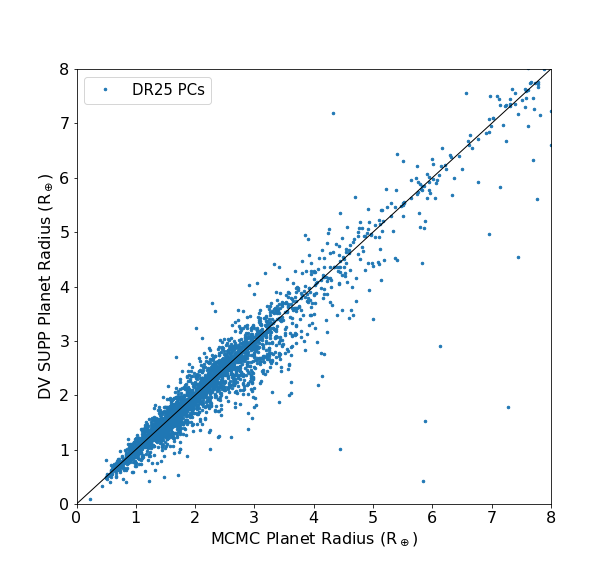
\includegraphics[width=0.99\linewidth]{fig-comparePradius-mcmcSup.png}
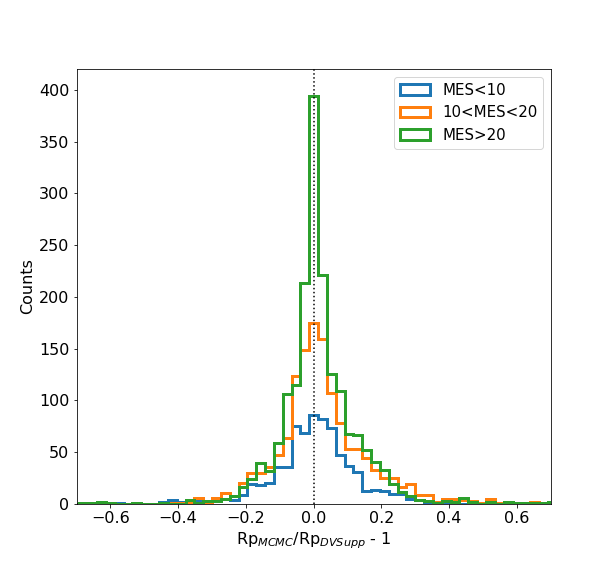
\includegraphics[width=0.99\linewidth]{fig-comparePradius-histogram.png}
\caption{Top: Comparison of the DR25 PCs fitted planet radii measured by the MCMC fits and the DV supplemental fits. The 1:1 line is drawn in black. Bottom: Histogram of the difference between the MCMC fits and the DV fits for the planet candidates in different MES bins. While individual objects have different fitted values, statistically the planet radii from the two fits agree. }
\label{f:mcmcsupp}
\end{figure}


\subsection{Stellar Catalog}
The derived parameters from transit fits (e.g. planetary radii and insolation flux) of the TCEs and KOIs rely critically on the accuracy of the stellar properties (e.g. radii, mass, temperature).   For all transit fits used by this catalog we use the DR25 Q1--Q17 stellar table provided by \citet{Mathur2017} which are based on conditioning published atmospheric parameters on a grid of Dartmouth isochrones \citet{Dotter2008}.  Typical uncertainties in this stellar catalog are $\approx$27 per cent in radius, $\approx$17 per cent in mass, and $\approx$51 per cent in density, which is somewhat smaller than previous catalogs. Because this information will continue to be updated (with data from missions such as Gaia \citet{Gaia2016}) we perform our vetting and analysis independent of stellar properties where possible, a notable exception being the limb darkening values needed for the transit fits.